\subsection{Устойчивость по линейному приближению.}
\begin{reminder}
    Все отображения считаются гладкими достаточное число раз, чтобы мы могли легально делать то, что делаем.
\end{reminder}
    Рассмотрим разложение по формуле Тейлора для автономной динамической системы $\dot{\bt{x}} = \bt{f}(\bt{x})$ с нулевым положением равновесия:
\[
    \dot{\bt{x}} = D_{\bt{0}}\bt{f} \cdot \bt{x} + O\big(\|\bt{x}\|^2\big), \bt{x} \ra \bt{0}.
\]
    Отбросим члены старшего порядка, обозначим $A = D_{\bt{0}}\bt{f}$ и будем рассматривать линеаризованную систему
\[
    \dot{\bt{x}} = A\bt{x}.
\]
    Характеристическим полиномом этой системы будем называть полином
\[
    P(\lambda) = \det (A - \lambda I).
\]
    Заметим, что если все собственные значения имеют неположительные вещественные части, то нулевое положение равновесия -- устойчиво, а если, к тому же, они все строго отрицательны, то положение равновесия является асимптотически устойчивым (в силу структуры решения системы линейных уравнений). \\
Пусть у нас есть теперь некоторая стационарная система, параметризованная $\{\bt{q}\}$, имеющая кинетическую энергию $T$ и вектор обобщённых сил $\bt{Q}$ (и нулевое положение равновесия).
Уравнения её движения определяются уравнениями Лагранжа:
\[
    \biggr(\dfrac{d}{dt}\dfrac{\partial}{\partial \bt{\dot{q}}} - \dfrac{\partial}{\partial \bt{q}}\biggr)T = \bt{Q}.
\]
В силу стационарности системы её кинетическая энергия является квадратичной формой относительно обобщённых скоростей:
\[
    T = \dfrac{1}{2}\dot{\bt{q}}A(\bt{q})\dot{\bt{q}}.
\]
Тогда линеаризованные уравнения Лагранжа (в окрестности нулевого положения равновесия) будут записаны в форме
\[
    A\ddot{\bt{q}} + B\dot{\bt{q}} + C\bt{q} = 0.
\]
Где введены следующие обозначения:
\[
    A = A(\bt{0}) \quad B = -\dfrac{\partial \bt{Q}}{\partial \dot{\bt{q}}}\biggr|_{\bt{\dot{q}, q} = \bt{0}} \quad  C = -\dfrac{\partial \bt{Q}}{\partial \bt{q}}\biggr|_{\bt{\dot{q}, q} = \bt{0}}.
\]
Характеристический полином этой системы определяется уравнением
\[
    P(\lambda) = \det (A\lambda^2 + B\lambda + C).
\]
\begin{theorem}[Ляпунов, об устойчивости по линейному приближению]
    Пусть дана автономная система $\dot{\bt{x}} = \bt{f}(\bt{x})$ с положением равновесия $\bt{x} = 0$ и $P(\lambda)$~---~характеристический полином её линеаризации в окрестности нуля.
    Тогда справедливы следующие утверждения:
    \begin{itemize}
        \item Если $P(\lambda)$~---~устойчив (то есть все собственные числа имеют отрицательную вещественную часть) то нулевое положение равновесия исходной системы асимптотически устойчиво.
        \item Если $P(\lambda)$ имеет хотя бы один корень с положительной вещественной частью, то нулевое положение равновесия исходной системы неустойчиво.
    \end{itemize}
\end{theorem}
Заметим, что справедливо следующее утверждение:
\begin{lemma}[на лекции была дана без доказательства]
    Пусть $A$~---~квадратная матрица над $\R$.
    Тогда верно следующее:
    \begin{itemize}
        \item Если все собственные значения $A$ имеют отрицательную вещественную часть то существует симметрическая положительно определённая матрица $B$ такая, что
        \[
            A^{T}B + B^{T}A = -I.
        \]
        \item Если есть хотя бы одно собственное значение с положительной вещественной частью, то существует симметрическая положительная определённая матрица $B$ такая, что
        \[
            A^T B + B^T A = I.
        \]
    \end{itemize}
\end{lemma}
\begin{note}[прим. техающего]
    Доказательство леммы можно найти в книге <<Теория матриц>>, Гантмахер.
\end{note}
Докажем теорему.
\begin{proof}
    Заметим, что производная в силу системы квадратичной формы $V = x^TBx$ вычисляется как
    \[
        \dot{V} = \dot{x}^T B x + x^T B \dot{x} = x^T A^T B x + x^T B A x = x^T (A^T B + B^T A) x = \pm x^T I x.
    \]
    (где знак перед производной мы выбираем исходя из того какой случай мы доказываем)
    Теперь, заметим, что мы можем взять в качестве функции Ляпунова (соответственно, функции Четаева) $V = x^T B x$~---~уже для исходной системы и получить
    \[
        \dot{V} = -\|\bt{x}\|^2 + O(\|\bt{x}\|^3), \bt{x} \ra \bt{0}.
    \]
    если все собственные значения матрицы $A$ имеют отрицательную вещественную часть и получить устойчивость нулевого решения по теореме Ляпунова.
    Или же
    \[
        \dot{V} = \|\bt{x}\|^2 + O(\|\bt{x}\|^3), \bt{x} \ra \bt{0}.
    \]
    если есть хотя бы один корень с положительной вещественной частью и получить неустойчивость нулевого положения равновесия по теореме Четаева.
\end{proof}
% Вот это всё речекнуть и дописать.
Известно, что справедлив критерий Рауса-Гурвица для устойчивости произвольного полинома.
\begin{theorem}[Раус-Гурвиц, на лекции была дана без доказательства]
    Пусть $P_m(\lambda) = a_m \lambda^m + \ldots a_0$ и, без ограничения общности, $a_m > 0$.
    Тогда следующие условия эквивалентны:
    \begin{enumerate}
        \item $P_m(\lambda)$~---~устойчив.
        \item Все диагональные миноры матрицы Гурвица $\Gamma$ положительны.
    \end{enumerate}
    Где под матрицей Гурвица понимается матрица следующего вида:
    \[
        \Gamma = \begin{pmatrix}
                     a_{m - 1} & a_{m - 3} & \ldots & 0 \\
                     a_m & a_{m - 2} & \ldots & 0 \\
                     0 & a_{m - 1} & a_{m - 3} & \ldots \\
                     0 & a_m & \ldots & 0 \\
                     \ldots & \ldots & \ldots & \ldots \\
                     0 & 0 & 0 & a_0
        \end{pmatrix}
    \]
\end{theorem}
Также справедлива следующая лемма:
\begin{lemma}[Необходимое условие устойчивости полинома]
    Если $P(\lambda)$~---~устойчив, то все его коэффициенты положительны.
\end{lemma}
\begin{example}[Бифуркация Пуанкаре-Четаева]
    Рассмотрим уравнение движения точки на прямой следующего вида:
    \[
        \ddot{x} + \dot{x} + x(\epsilon - x^2) = 0.
    \]
    Характеристическое уравнение линеаризованной системы
    \[
        \lambda^2 + \lambda + \epsilon = 0.
    \]
    имеет корни $\lambda_{1, 2} = \dfrac{-1 \pm \sqrt {1 - 4\epsilon}}{2}$.
    По теореме Ляпунова при $\epsilon > 0$ равновесие будет асимптотически устойчивым, а при $\epsilon < 0$ равновесие будет неустойчивым.
    Если же $\epsilon = 0$ то при помощи теоремы Ляпунова об устойчивости по линейному приближению мы ничего сказать не можем, поскольку корнями системы будут $\lambda_1 = 0, \lambda_2 = -1$.
    Но мы можем взять в качестве функции Ляпунова $V = \dfrac{\dot{x}^2}{2} - \dfrac{x^4}{4}$ и увидеть неустойчивость нулевого положения равновесия системы. \\
    Заметим, что при $\epsilon > 0$ появляются ещё два равновесия системы: $x = \pm \sqrt {\epsilon}$.
    Они будут неустойчивыми.
    Таким образом, бифуркационная диаграмма будет иметь следующий вид:
    \begin{figure*}[h!]
        \centering
        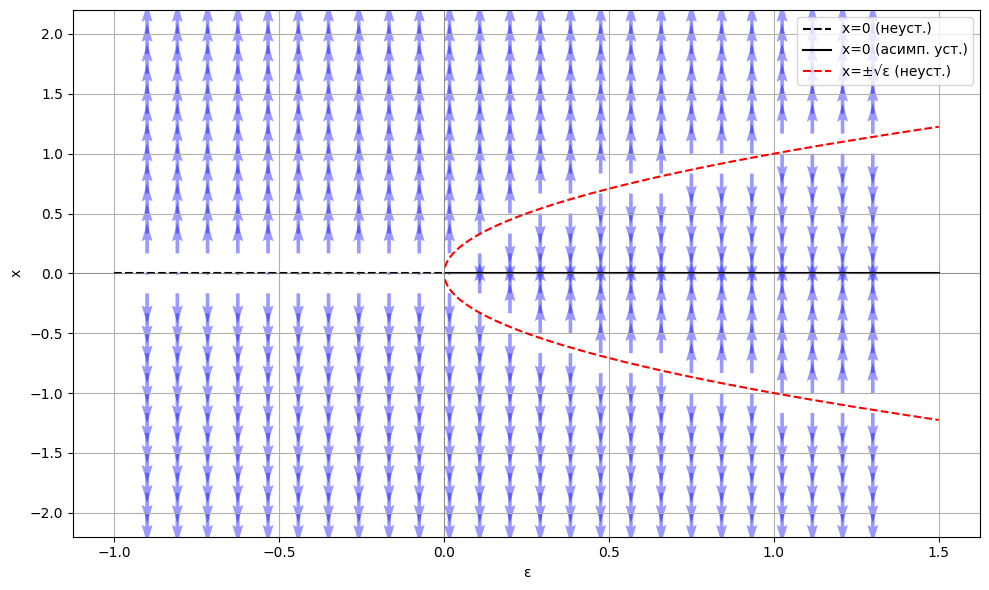
\includegraphics[width=0.8\linewidth]{images/poincarechetaevbifurcation}
        \caption{Бифуркация Пуанкаре-Четаева.}
    \end{figure*}
\end{example}
\begin{example}[Бифуркация Андронова-Хопфа]
    Рассмотрим точку на прямой, уравнения движения которой подчиняются следующему дифференциальному уравнению:
    \[
        \ddot{x} + \epsilon \dot{x} + x(1 - x\dot{x}) = 0.
    \]
    Характеристическое уравнение линеаризованной системы имеет вид
    \[
        \lambda^2 + \epsilon \lambda + 1 = 0.
    \]
    И, соответственно, корни $\lambda_{1, 2} = \dfrac{-\epsilon \pm \sqrt {\epsilon^2 - 4}}{2}$. \\
    Согласно теореме Ляпунова об устойчивости по первому приближению при $\epsilon > 0$ нулевое положение равновесия устойчиво, а при $\epsilon < 0$ -- неустойчиво; при $\epsilon = 0$ мы ничего про его устойчивость сказать не можем. \\
    Перепишем уравнение системы в виде
    \[
        \begin{cases}
            \dot{x} = y \\
            \dot{y} = - \epsilon y - x(1 - xy).
        \end{cases}
    \]
    И перейдём к полярным координатам:
    \[
        \begin{cases}
            x = r \cos \phi \\
            y = r \sin \phi.
        \end{cases}
    \]
    Система переписывается как
    \[
        \begin{cases}
            \dot{r} = -\epsilon r \cos^2 \phi + r^3 \sin^2 \phi \cos^2 \phi \\
            \dot{\phi} = 1 + \epsilon \sin \phi \cos \phi - r^2 \sin^3 \phi \cos \phi.
        \end{cases}
    \]
    Полагая $r = \rho \sqrt {\epsilon}$ окончательно имеем
    \[
        \begin{cases}
            \dot{\rho} = \epsilon \rho \cos^2\phi (\rho^2 \sin^2 \phi - 1) \\
            \dot{\phi} = 1 + \epsilon \sin \phi \cos \phi (1 - \rho^2 \sin^2 \phi).
        \end{cases}
    \]
    Усредним систему по $\phi$ и получим
    \[
        \begin{cases}
            \dot{\rho} = \dfrac{\epsilon \rho (\rho^2 - 4)}{8} \\
            \dot{\phi} = 1.
        \end{cases}
    \]
    Эта система имеет периодическое решение при $\rho = 2$ и $\phi = t$ с периодом $2\pi$.
    После перехода обратно к полярным координатам это будет неустойчивый предельный цикл, близкий к окружности радиуса $r = 2\sqrt {\epsilon}$.
\end{example}
\subsection{Устойчивость положения равновесия консервативных систем.}
Пусть дана некоторая консервативная механическая система с кинетической энергией $T$ и потенциалом $\Pi$.
Её уравнения Лагранжа могут быть записаны как
\[
    \biggr(\dfrac{d}{dt}\dfrac{\partial}{\partial \dot{\bt{q}}} - \dfrac{\partial}{\partial \bt{q}}\biggr)T = -\dfrac{\partial \Pi}{\partial \bt{q}}.
\]
С учётом того, что равновесие -- стационарная точка потенциала, мы можем считать $T$ и $\Pi$ в окрестности нуля равными
\[
    T = \dfrac{1}{2}\dot{\bt{q}}A\dot{\bt{q}}, \quad \Pi = \dfrac{1}{2}\bt{q}C\bt{q}.
\]
где под $A$ понимается матрица квадратичной части кинетической энергии в нуле, а $C = \Hess \Pi = \dfrac{\partial^2 \Pi}{\partial \bt{q}\partial \bt{q}}$.
Тогда уравнения Лагранжа запишутся как
\[
    A\ddot{\bt{q}} + C\bt{q} = 0.
\]
Поскольку матрицы $A$ и $C$ -- симметричны и $A$ -- положительно определённая матрица, то существует базис $\bt{\theta}$ в котором обе матрицы имеют диагональный вид.
Более того, мы можем потребовать чтобы $A$ в нём была равна $I$, и тогда на диагонали матрицы $\Lambda$ (то есть матрицы $C$ в базисе $\bt{\theta}$) будут стоять собственные числа системы.
В базисе $\bt{\theta}$ уравнения Лагранжа записываются как
\[
    I\ddot{\bt{\theta}} + \Lambda \bt{\theta} = 0.
\]
И система распалась на $n$ независимых осцилляторов:
\[
    \ddot{\theta}_k + \lambda_k \theta_k = 0.
\]
\begin{theorem}[Ляпунова, о неустойчивости]
    Консервативная система с нулевым положением равновесия неустойчива в нём если гессиан потенциала в нуле имеет хотя бы одно отрицательное собственное значение.
\end{theorem}
\begin{proof}
    Из вида уравнений Лагранжа следует что характеристическим полиномом системы является
    \[
        \prod (\lambda^2 + \lambda_k) = 0.
    \]
    Таким образом, если $\exists k \hookrightarrow \lambda_k < 0$ то у системы есть собственное число с положительной вещественной частью и нулевое равновесие будет неустойчиво по теореме Ляпунова об устойчивости по первому приближению.
\end{proof}
\begin{theorem}
    Если консервативная механическая система имеет устойчивое равновесие в силу теоремы Лагранжа-Дирихле, то добавление гироскопических или диссипативных сил оставит равновесие устойчивым.
\end{theorem}
\begin{proof}
    Мощность $\dot{E}_{\text{гир}} = 0$, $\dot{E}_{\text{дис}} \leq 0$, а следовательно это так по теореме Ляпунова об устойчивости: мы точно также можем взять энергию в качестве функции Ляпунова.
\end{proof}
\begin{theorem}
    Если консервативная механическая система имеет устойчивое равновесие в силу теоремы Лагранжа-Дирихле, то добавление сил полной диссипации делает систему асимптотически устойчивой.
\end{theorem}
\begin{proof}
    В силу теоремы об устойчивости по линейному приближению это будет так, поскольку характеристический полином системы станет устойчивым.
\end{proof}
\subsection{Малые колебания в окрестности положения равновесия.}
Предположим что $C$ -- тоже положительно определённая матрица и тогда $\bt{0}$ -- устойчивое положение равновесия.
Уравнение
\[
    A \ddot{\bt{q}} + C\bt{q} = 0.
\]
будем называть уравнением малых колебаний. \\
Собственные числа $\Lambda$ являются корнями следующего полинома:
\[
    P(\lambda) = \det (C - \lambda A).
\]
А уравнение $P(\lambda) = 0$ называется вековым уравнением частот.
Для всякого $k$ и $\lambda_k$ амплитудным вектором будем называть такой $\bt{u}^k$, что
\[
    (C - \lambda_k A)\bt{u}^k = 0.
\]
Заметим, что матрица
\[
    U = \begin{pmatrix*} \bt{u}^1 & \ldots & \bt{u}^n
    \end{pmatrix*}.
\]
является матрицей перехода к нормальным координатам, если к тому же $(\bt{u}^i)^T A \bt{u}^j = \delta^{ij}$ (то есть амплитудные вектора отнормированы).
Поскольку в нормальных координатах уравнения движения имеют вид
\[
    \ddot{\theta_k} + \lambda_k \theta_k = 0.
\]
То решением для $\theta_k$ будет
\[
    \theta_k(t) = C_k \sin (\sqrt {\lambda_k} t +\alpha_k).
\]
А значит общее движение системы записывается как
\[
    \bt{q}(t) = U\bt{\theta}(t).
\]